%% Submissions for peer-review must enable line-numbering 
%% using the lineno option in the \documentclass command.
%%
%% Preprints and camera-ready submissions do not need 
%% line numbers, and should have this option removed.
%%
%% Please note that the line numbering option requires
%% version 1.1 or newer of the wlpeerj.cls file, and
%% the corresponding author info requires v1.2

\documentclass[fleqn,10pt,lineno]{wlpeerj} % for journal submissions
% \documentclass[fleqn,10pt]{wlpeerj} % for preprint submissions

\title{Allometric growth parameters for invasive lionfish \emph{Pterois
volitans} (Actinopterygii, Scorpaenidae) in the Western Atlantic}

\author[1]{Juan Carlos Villaseñor-Derbez}
\affil[1]{Bren School of Environmental Sciences and Management, University of
California Santa Barbara, Santa Barbara, California, U.S.}
\corrauthor[1]{Juan Carlos Villaseñor-Derbez}{jvillasenor@bren.ucsb.edu}

% \keywords{Keyword1, Keyword2, Keyword3}

\begin{abstract}
Lionfish (\emph{Pterois volitans/miles}) are an invasive species in the
North-Western Atlantic and the Caribbean. In order to better manage the
invasion, inform lionfish removal programs, and estimate biomass
available for harvest, we must be able to accurately estimate their
total biomass, frequently from length observations. This work compares
length-weight relationships of the invasive lionfish through the
invasion range and reports the length--weight relationship for lionfish
in the Central Mexican Caribbean. A review of 13 length--weight
relationships reported in eight peer-reviewed studies and FishBase is
provided. These parameters were used to identify spatial variation in
weight-at-length. For a given length, parameters from the Caribbean
yielded lower weights than those from the Gulf of Mexico and Atlantic,
indicating that weight-at-length is spatially variable. This highlights
the importance of using site-specific parameters to estimate biomass
from length observations. This study also reports a new pair of
length-weight parameters (\(a = 3.2056 imes 10^{-6}; b = 3.235\)) for
organisms sampled in the Central Mexican Caribbean. Findings from this
work can aid managers and decision makers to better select length-weight
parameters when these are not available for their region of interest.
\end{abstract}

\usepackage{amsthm}
\newtheorem{theorem}{Theorem}[section]
\newtheorem{lemma}{Lemma}[section]
\theoremstyle{definition}
\newtheorem{definition}{Definition}[section]
\newtheorem{corollary}{Corollary}[section]
\newtheorem{proposition}{Proposition}[section]
\theoremstyle{definition}
\newtheorem{example}{Example}[section]
\theoremstyle{definition}
\newtheorem{exercise}{Exercise}[section]
\theoremstyle{remark}
\newtheorem*{remark}{Remark}
\newtheorem*{solution}{Solution}
\begin{document}

\flushbottom
\maketitle
\thispagestyle{empty}

\section{Introduction}\label{introduction}

At least 84\% of the marine eco-regions have reported the presence of an
invasive species \citep{molnar_2008}. These represent a major threat to
local biodiversity and the economic activities that depend on it, like
tourism or fisheries \citep{bax_2003}. Invasive species may also
threaten native species through competition \citep{davis_2003} or
predation. By 2005, the economic cost of invasive species to the United
States was estimated at \$120 billion per year and nearly 42\% of
species that have been included in the Endangered or Threatened species
list have been labeled as such due to presence of invasive species
\citep{pimentel_2005}. This highlights the importance of understanding,
managing, and preventing ecological invasions.

Lionfish (\emph{Pterois volitans/miles} complex) are an invasive species
in the North-Western Atlantic and the Caribbean, likely introduced
through liberation of aquarium-kept organisms \citep{betancurr_2011}.
They are the first marine vertebrates to establish in North Atlantic
\citep{schofield_2009,schofield_2010} and Caribbean coasts
\citep{sabidoitza_2016}. Lionfish have been widely reported in coral
reefs \citep{aguilarperera_2010}, but also in other habitats such as
estuaries \citep{jud_2011}, mangroves \citep{barbour_2010}, areas with
hard-bottoms \citep{muoz_2011}, and mesophotic reefs
\citep{andradibrown_2017}. Due to its threat to local biodiversity, the
speed of their spread, and its difficulty of management, their presence
in these waters has been labeled as a major marine invasion
\citep{hixon_2016}.

A significant amount of research has been done to describe lionfish
feeding ecology in North Carolina \citep{muoz_2011}, the Bahamas
\citep{morris_2009,cote_2013}, Northern Gulf of Mexico
\citep{dahl_2014}, Mexican Caribbean
\citep{valdezmoreno_2012,villaseorderbez_2014}, Belize
\citep{hackerott_2017}, and Costa Rica \citep{sandel_2015}. Their
feeding behavior and high consumption rates can reduce recruitment
\citep{albins_2008} and population sizes \citep{green_2012} of native
reef-fish species, and further the endangerment of critically endangered
reef fish \citep{rocha_2015}. (However, see \citet{hackerott_2017} for a
case where there was no evidence that lionfish affected the density,
richness, or composition of prey fishes). Major efforts have also been
made to understand the possible impacts of the invasion by keeping track
of its range through time \citep{schofield_2009,schofield_2010} and
predicting invasion ranges under climate change scenarios
\citep{grieve_2016}. By combining information from these disciplines,
researchers have been able to predict the trophic impacts of lionfish
\citep{ariasgonzalez_2011}, which can then be translated into
ecosystem-level and economic impacts.

Seeking to reduce lionfish densities, governments and non-profit
organizations have promoted removal programs and incentivized its
consumption \citep{chin_2016}. In some cases, these have shown to
significantly reduce -but not quite eliminate- lionfish abundances at
local scales \citep{sandel_2015,chin_2016,deleon_2013}. The rapid
recovery rates exhibited by lionfish \citep{barbour_2011} and the
persistent populations in mesophotic coral ecosystems
\citep{andradibrown_2017} -which can contribute with recruitment to
shallow-water populations- make of complete eradication through fishing
effort an unlikely solution. However, further incentivizing its
consumption might create a demand big enough to promote and sustain a
stable fishery \citep{chin_2016}, which can reduce local abundances and
control -not eradicate- the invasion while providing alternative
livelihoods.

The feasibility of lionfish removal programs has been extensively
evaluated through field
observations\citep{usseglio_2017,sandel_2015,chin_2016,deleon_2013} and
empirical modeling \citep{barbour_2011,morris_2011,johnston_2015}. The
latter measure changes in biomass or density
\citep{barbour_2011,johnston_2015} in response to increased mortality
(\emph{i.e.} lionfish removal). In this case, biomass represents the sum
of all fish's individual weight. Total Weight (TW) can be estimated from
Total Length (TL) observations using the allometric growth equation
(\(TW = aTL^b\)). Parameters \(a\) and \(b\) for this equation exist for
North Carolina \citep{barbour_2011}, Northern \citep{fogg_2013} and
Southern Gulf of Mexico \citep{aguilarperera_2016}, the Southern Mexican
Caribbean \citep{sabidoitza_2016}, Little Cayman \citep{edwards_2014},
Jamaica \citep{chin_2016}, Bonaire \citep{deleon_2013} and Costa Rica
\citep{sandel_2015}, but remain unavailable for the central Mexican
Caribbean. The weight-at-length of a species can vary across regions as
a response to biotic (\emph{e.g.} local food availability) and abiotic
(\emph{e.g.} water temperature) conditions \citep{johnson_2016}. Thus,
when using biomass-informed models or estimating biomass from length
observations, it is important to use site-specific parameters to obtain
an accurate estimate. This is especially important when research
involves identifying the total biomass available for harvest by fishers
\citep{chin_2016} or the efficacy of lionfish removals
\citep{barbour_2011,morris_2011,johnston_2015}.

Here, I provide the first allometric growth parameters for the invasive
lionfish in the central Mexican Caribbean region. At the same time, I
highlight the importance of using site-specific parameters by estimating
biomass with parameters from other regions across the invasion range and
comparing them to observed biomass. I also provide other 13 standardized
parameters from eight studies through the invasion range, making them
readily accessible for future research. Finally, I discuss the way in
which allometric parameters are reported, and call for standardization
to facilitate their use.

\clearpage

\section{Materials and Methods}\label{materials-and-methods}

\emph{Area of study}

The study took place off the coasts of Playa del Carmen, in the Mexican
Caribbean Figure \ref{fig:map}. The region represents the northernmost
section of the Mesoamerican Barrier Reef System \citep{ruizzarate_2004}.
Coral reefs and mangroves are locally important habitats that represent
important sources of income in terms of extractive (\emph{e.g.}
recreational fishing) and non-extractive (\emph{e.g.} SCUBA diving)
activities related to tourism, the main source of income to the local
economy \citep{murray_2007}.

The reef profile has been described by \citet{ariasgonzalez_1998},
indicating that the reef lagoon extends about 500 m from the coast,
until the reef crest is reached. The reef becomes deeper, leading to the
reef front often found at 700 m from the coastline and extends for an
additional 300 m. At approximately 1000 m away from shore and 30 - 40 m
depth, the reef leads to a drop-off. Along a perpendicular profile to
the coast, bands of reef are interrupted by sand patches at 8 - 12 m
deep and 16-18 m deep. Along the coast, these reefs have been reported
to be under significant anthropogenic pressure, likely causing a shift
in structure and function \citep{bozec_2008}.

\begin{figure}
\centering
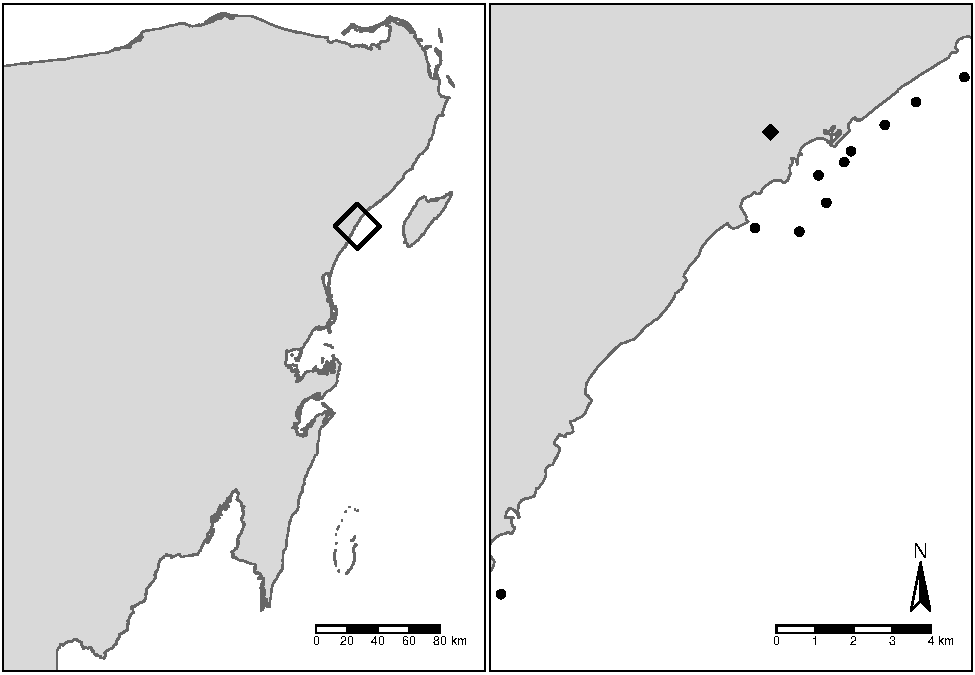
\includegraphics{Manuscript_files/figure-latex/unnamed-chunk-1-1.pdf}
\caption{\label{fig:unnamed-chunk-1}\label{fig:map}Map of the study area.
The black inset on the left (Yucatan Peninsula) indicates the location
where study sites are distributed. On the right, circular markers
indicate sampling sites and the black romboid indicates location of
Puerto Aventuras, Mexico.}
\end{figure}

\emph{Fish sampling}

A total of 33 SCUBA immersions were performed in 10 sampling sites along
the coast in 2010 (Fig. 1, Table I). Sampling locations included wall
and carpet reefs at depths between 5.7 m and 38.1 m. All observed
organisms (n = 109) were collected using hand nets and numbered
collection bottles. The use of hand nets prevented any weight loss due
to bleeding and allowed a better representation of small sizes, often
ignored due to gear selectivity when spearing. Organisms were euthanized
and frozen within 30 minutes of completing the dive and stored for
posterior analysis. Total Length (TL; mm) and Total Weight (TW; gr) were
recorded for all organisms.

\begin{table}

\caption{(\#tab:table of locations)Coordinates, minimum, maximum and mean depth (m), and number of samples for each location.}
\centering
\begin{tabular}[t]{llllllr}
\toprule
Location & Lat. & Long. & Min. Depth & Max. Depth & Mean Depth & n\\
\midrule
Canones & 20.477 & -87.233 & 15.0 & 31.2 & 21.6 & 11\\
Castillo & 20.496 & -87.220 & 12.5 & 30.5 & 27.5 & 18\\
Cuevitas & 20.478 & -87.244 & 7.4 & 12.8 & 11.2 & 4\\
Islas & 20.490 & -87.228 & 14.0 & 19.4 & 16.7 & 10\\
Paamul & 20.513 & -87.192 & 9.9 & 22.7 & 15.5 & 31\\
\addlinespace
Paraiso & 20.484 & -87.226 & 9.4 & 38.1 & 17.7 & 16\\
Pared & 20.502 & -87.212 & 12.1 & 21.0 & 16.3 & 12\\
Pedregal & 20.507 & -87.204 & 14.4 & 14.9 & 14.7 & 3\\
Santos & 20.493 & -87.222 & 5.7 & 26.6 & 16.2 & 2\\
Tzimin-Ha & 20.393 & -87.307 & 21.2 & 24.6 & 22.9 & 2\\
Total &  &  & 5.7 & 38.1 & 18.6 & 109\\
\bottomrule
\end{tabular}
\end{table}

\emph{Data analysis}

The weight at length relationship between the observed variables is
described by the allometric growth function:

\begin{equation}
\label{eq:allometric}
TW = aTL^b
\end{equation}

Where \(TW\) is the Total Weight (gr), \(TL\) is the Total Length (mm),
\(a\) is the ponderal index and \(b\) is the scaling exponent or
allometric parameter. When \(b = 3\), it is said that the organism
exhibits a perfect isometric growth. The dependent and independent
variables were transformed via base-10 logarithms, thus the equation
becomes:

\begin{equation}
\label{eq:log-alo}
log_{10}(TW) = b\times log_{10}(TL) + log{10}(a)
\end{equation}

This can be simplified and re-written as:

\begin{equation}
\label{eq:log-alo-trans}
Y = mX + c
\end{equation}

Where \(Y = log_{10}(TW)\), \(X = log_{10}(TL)\), \(m = b\), and
\(c = log_{10}(a)\). Since \(b = m\), we will only use \(b\) throughout
the paper for simplicity. The coefficients (\(c\) and \(b\)) were
estimated with an Ordinary Least Square Regression and
heteroskedastic-robust standard error correction was performed. Both
coefficients were tested against the null hypothesis of no change
(\emph{i.e.} \(H_0: c = 0\) and \(H_0: b = 0\)). Additionally, the
allometric parameter was tested against the null hypothesis of isometric
growth (\(H_0: b = 3\)). Coefficients were tested with a two-tailed
Student's t-test. The significance of the regression was corroborated
with an F-test.

Other length-weight relationships (n = 13) were extracted from
peer-reviewed literature. Parameters were obtained for North Carolina
{[}n = 1,barbour\_2011{]}, Northern {[}n = 3,fogg\_2013{]} and Southern
Gulf of Mexico {[}n = 3,aguilarperera\_2016{]}, the Southern Mexican
Caribbean {[}n = 1,sabidoitza\_2016{]}, Little Cayman {[}n =
1,edwards\_2014{]}, Jamaica {[}n = 1,chin\_2016{]}, Bonaire {[}n =
1,deleon\_2013{]} and Costa Rica {[}n = 1,sandel\_2015{]} and Fishbase
{[}n = 1,froese\_website\_2016{]} were also included. When available,
information on sampling methods, gender differentiation, location, and
depth ranges of each study was retrieved. Whenever gender was not
specified, it was assumed that the results were presented for pooled
genders.

During the review process, some papers indistinctly used \(a\) to report
either the ponderal index in eq. 1 or the y-intercept (\(c\)) in eq. 3,
which might sometimes be overlooked. Furthermore, some studies reported
their parameters as mm-to-gr conversions, but a rapid evaluation of such
parameters indicated that they were estimated as cm-to-gr conversions.
Here, all parameters are reported as TL(mm) to TW(gr) conversions. When
required, values from other studies were transformed for consistency.

Since uncertainty arround estimated relationships was not reported in
some of the reviewed studies, it was not possible to test for
statistical differences between relationships. Instead, the 13
length-weight relationships were usd to calculate expected weight for
the organisms sampled in the Central Mexican Caribbean (n = 109).
Expected weights were divided by the observed weights to obtain a ratio.
Difference in mean weight ratios across studies were tested with a
one-way Analysis of Variance (ANOVA).

All hypothesis testing was performed with an \emph{a priori} confidence
level of \(\alpha = 0.01\) in R version 3.4.0 \citep{rcore_2017}. Data
wrangling was done with the tidyverse package \citep{tidyverse_2017}.
Maps were created with a mix of functions from the sp \citep{sp_2017},
rgdal \citep{rgdal_2017}, tmap \citep{tmap_2017}, and tmaptools
\citep{tmaptools_2017} packages. Heteroskedastic-robust standard errors
were calculated with the sandwich \citep{sandwich_2014} and lmtest
\citep{lmtest_2002} packages. Models were manipulated with the broom
package \citep{broom_2017}. Raw data and code used in this work is
available at github.com/jcvdav/lionfish\_biometry.

\section{Results}\label{results}

Organism TL ranged between 34 and 310 mm and TW between 0.3 and 397.7
gr. The smallest organism (TL = 34.00 mm) was also the lightest organism
(TW = 0.30 gr). However, the largest organism (TL = 310.00 mm) was not
the heaviest (TW = 303.70 gr), and the heaviest organism (TW = 397.70
gr) was 292.00 mm in total length. Kernell density plots (Fig. 2) show
the distribution for TL and TW for all sampled organisms. Both measures
were positively skewed, with skewness of 0.87 for TL and 2.25 for TW.

\begin{figure}
\centering
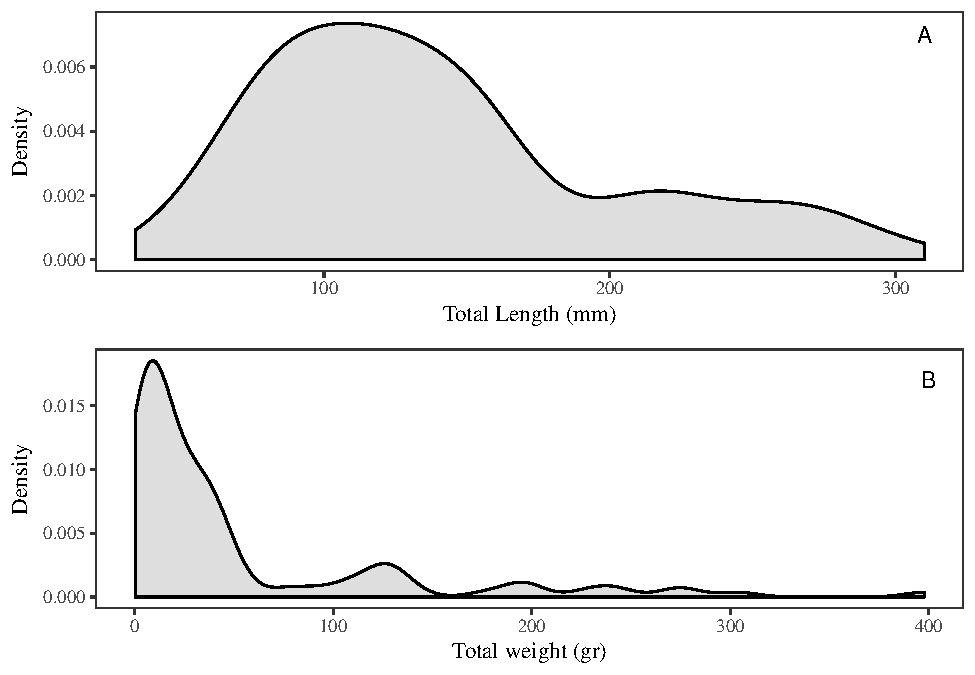
\includegraphics{Manuscript_files/figure-latex/histogram figures-1.pdf}
\caption{(\#fig:histogram figures)Kernell density plots for a) Total
length (mm) and b) Total weight (gr) for 109 lionfish sampled in the
central Mexican Caribbean.}
\end{figure}

\emph{Length-weight relationship}

The model adjusted to eq. 3 estimated the coefficient values at
\(b = 3.2347391\) and \(c = -5.4940866\). Thus, TW (gr) can be
calculated from TL (mm) as a linear equation:
\(log_{10}(TW) = 3.2347391\times log_{10}(TL) -5.4940866\), or its
exponential form: \(TW = 3.2056297\times 10^{-6}\times TL^{3.2347391}\).
The intercept (\(c\)) and slope \((b)\) were significantly different
from zero (\(t(107) = -66.17; p<0.01\) and \(t(107) = 83.24; p<0.01\),
respectively), rejecting the null hypothesis of no change. Additionally,
the allometric factor (\(b\)) was significantly different from the value
of isometric growth of \(b = 3\) (\(t(107) = 6.04; p<0.01\)), indicating
that lionfish present allometric growth. More information on model fit
and confidence intervals for the estimated coefficients is presented in
Table II. The relationship between Total Length and Total Weight is
presented in Figure 3.

\begin{figure}
\centering
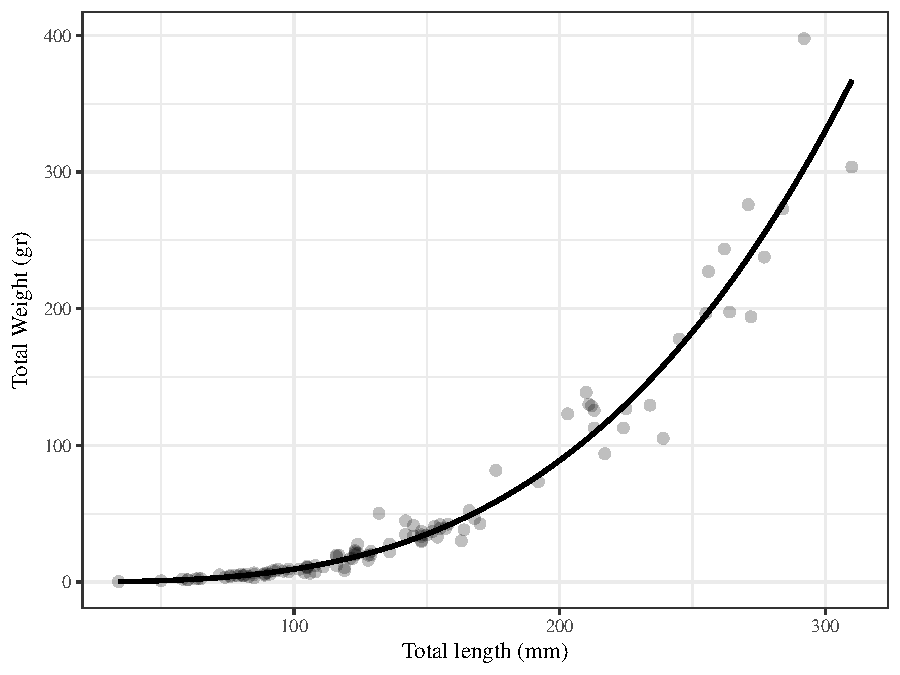
\includegraphics{Manuscript_files/figure-latex/scatter plot-1.pdf}
\caption{(\#fig:scatter plot)Length-weight relationship for 109 lionfish
sampled in the central Mexican Caribbean. Points indicate samples, solid
line indicates curve of best fit.}
\end{figure}

\begin{table}[!htbp] \centering 
  \caption{Regression table for the linear model fit between log10-transformed Total Weight (dependent variable) and Total Length (independent variable). Numbers in parentheses next to coefficient estimates indicate heteroskedastic-robust standard errors.} 
  \label{} 
\begin{tabular}{@{\extracolsep{5pt}}lc} 
\\[-1.8ex]\hline 
\hline \\[-1.8ex] 
 & \multicolumn{1}{c}{\textit{Dependent variable:}} \\ 
\cline{2-2} 
\\[-1.8ex] & log10(TW) \\ 
\hline \\[-1.8ex] 
 c & $-$5.494 (0.083)$^{***}$ \\ 
  b & 3.235 (0.039)$^{***}$ \\ 
 \hline \\[-1.8ex] 
95\% CI for c & (-5.657--5.331) \\ 
85\% CI for b & (3.159-3.311) \\ 
F Statistic & 6928.67*** (df = 1; 107) \\ 
Observations & 109 \\ 
Adjusted R$^{2}$ & 0.976 \\ 
Residual Std. Error & 0.096 (df = 107) \\ 
\hline 
\hline \\[-1.8ex] 
\textit{Note:}  & \multicolumn{1}{r}{$^{*}$p$<$0.1; $^{**}$p$<$0.05; $^{***}$p$<$0.01} \\ 
\end{tabular} 
\end{table}

\emph{Comparison of allometric parameters}

From the eight peer-reviewed studies including information on growth
parameters for \emph{P. volitans} and Fishbase
\citep{froese_website_2016}, 13 parameters were identified (Table III).
Two studies \citep{aguilarperera_2016,fogg_2013} reported gender-level
and pooled parameters, while the rest presented pooled results. The
smallest coefficient of determination was presented by \citet{chin_2016}
with \(R^2 = 0.8715\), while \citet{sabidoitza_2016} reported the
highest value at \(R^2 = 0.9907\). Reviewed studies presented
information for organisms obtained at depths between 0.5 and 57 m. Two
studies \citep{aguilarperera_2016,chin_2016} explicitly stated that
their organisms were sampled with pole spears. Five studies
\citep{sandel_2015,barbour_2011,fogg_2013,edwards_2014,sabidoitza_2016}
mentioned that some of their organisms were obtained with pole spears
(or other type of harpoon). A single study \citep{deleon_2013} did not
specify how organisms were sampled.

Parameters from models fit to males or females exclusively tend to have
a higher steepness (\emph{i.e.} higher allometric parameter), with mean
\(\pm\) standard deviation values of \(b = 3.27 \pm 0.06\) and
\(b = 3.31 \pm 0.23\) for males and females respectively, compared to
parameters from models for pooled genders with a mean \(\pm\) standard
deviation value of \(b = 3.09 \pm 0.22\). In the case of the ponderal
index (\(a\)) and its \(log_{10}\) transformed parameter (\(c\)), values
were higher for parameters for pooled genders. Figure 4 shows the
predicted weights for organisms within the size range of these study
using the 14 parameters previously described.

\begin{figure}
\centering
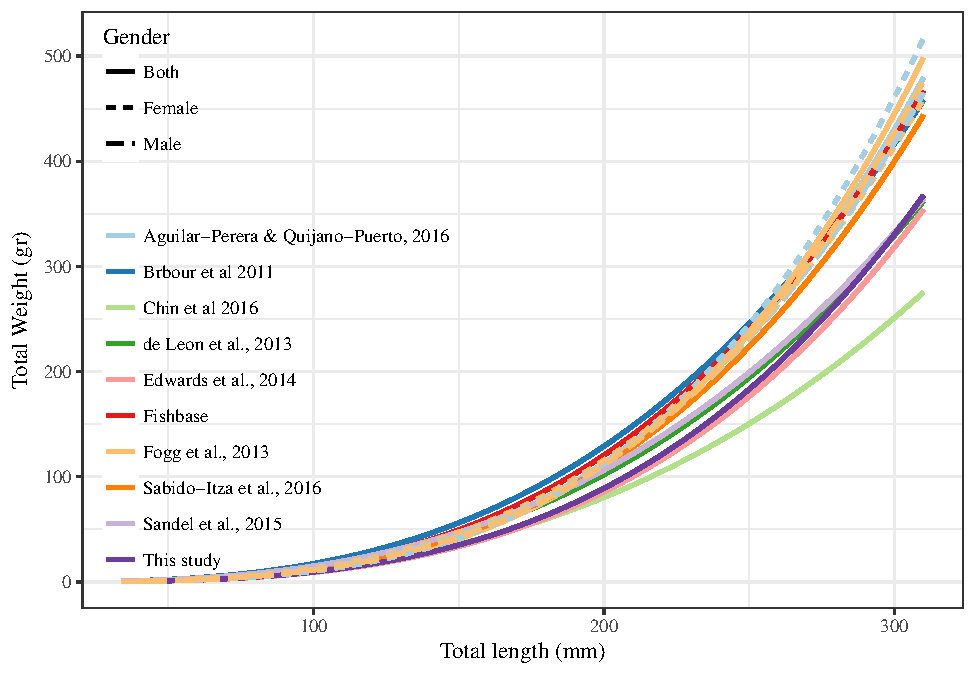
\includegraphics{Manuscript_files/figure-latex/review plots-1.pdf}
\caption{(\#fig:review plots)Length-weight relationships (n = 14) for
eight studies, this study, and Fishbase. Colors indicate studies from
which the parameters were extracted. Solid lines indicate that the fit
was performed for males and females pooled together. Dotted lines
indicate that the regression was performed on females, and dashed lines
indicate it was performed for males.}
\end{figure}

There were significant differences in expected-to-observed weight ratios
estimated for each pair of parameters (F(13, 1512) = 39.28; p
\textless{} 0.05). From all allometric parameters reviewed, those of
\citet{edwards_2014} provided the lowest weight estimates, with an
expected-to-observed weight ratio of 0.98 \(\pm\) 0.23 (mean \(\pm\)
SD). On the other hand,barbour\_2011 yielded the highest weight
estimates, with a mean (\(\pm\) SD) expected-to-observed weight ratio of
1.76 \(\pm\) 0.50. Predicted-to-observed weight ratios and groups
identified by Tukey's HSD (\(\alpha = 0.05\)) are presented in Figure 5.

\begin{figure}
\centering
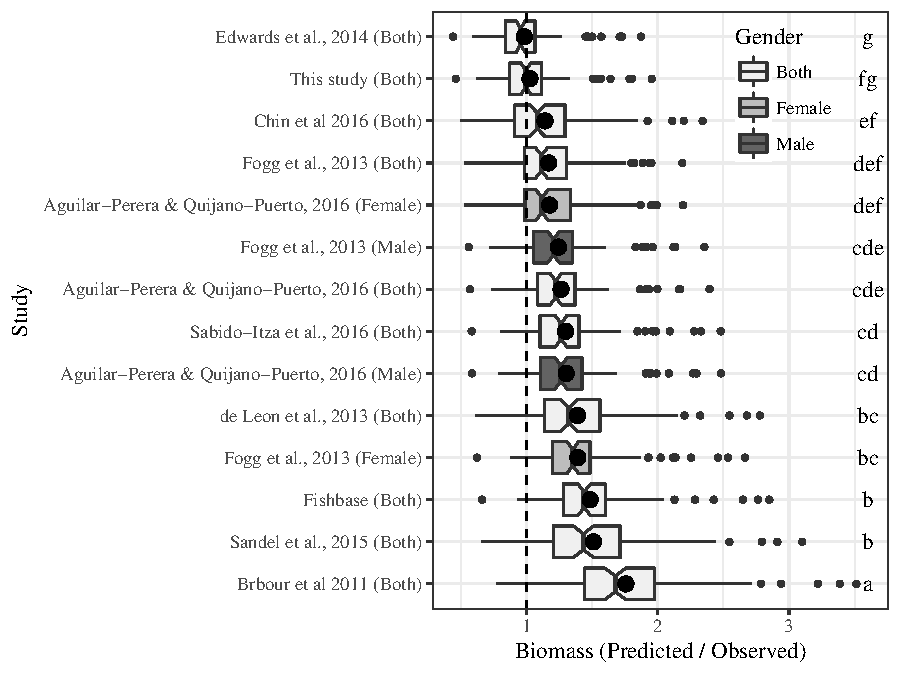
\includegraphics{Manuscript_files/figure-latex/plot comparing predictions-1.pdf}
\caption{(\#fig:plot comparing predictions). Box and whiskers plot
showing the distribution of predicted to observed biomass ratios for 14
pairs of allometric parameters. Lines indicate median values, circles
indicate mean values, notches represent 95\% confidence intervals
arround the median, lower and upper hinges correspond to the first and
third quartiles, whiskers extend to the largest and lowes values within
1.5 inter-quartile range of the hinge, small points represent outliers
further away than the whiskers. Like letters indicate values that do not
differ significantly (Tukey's HSD; p \textless{} 0.05).}
\end{figure}

\section{Discussion}\label{discussion}

This study provides the first pair of allometric growth parameters
specific to the Central Mexican Caribbean, complementing other studies
performed in Mexican waters in the Alacranes Reef
\citep{aguilarperera_2016} and Xcalak National Park
\citep{sabidoitza_2016}. By using hand nets instead of spears, we are
able to sample a wider range of sizes often ignored by pole spear
samples, allowing us to include smaller organisms. Estimating parameters
by including smaller organisms ensures better estimation of weight for
smaller sizes. This is especially important when biomass is calculated
from visual census, where small organisms can be registered. Thus, this
study also increases certainty in weight estimation of small organisms.

The length-weight coefficients estimated in this study were within the
range identified by studies in other regions
\citep{barbour_2011,fogg_2013,aguilarperera_2016,sabidoitza_2016,edwards_2014,chin_2016,deleon_2013,sandel_2015}.
However, the ones presented here provide lower weight estimates for a
same length. Until about TL = 200 mm, there are no appreciable
differences between the parameters for organisms from the Mexican
Caribbean and those for little Cayman \citep{edwards_2014} and Jamaica
\citep{chin_2016}. Yet, for larger organisms (TL \textgreater{} 270 mm)
parameters from Costa Rica \citep{sandel_2015} and Bonaire
\citep{deleon_2013} provide similar estimates to those from this study.
Conversely, these same studies tend to estimate higher weights ---as
compared to the ones reported here--- for smaller organisms, likely due
to the lack of small organisms in the samples used to estimate their
parameters. When ever possible, future works should consider the use of
hand nets to obtain the samples not only for studies on
weight-at-length, but also diet, behavior and life history, where length
can be an important factor.

There are evident differences in weight-at-length between organisms from
the Caribbean and Gulf of Mexico / North-Western Atlantic. Weight
estimates with parameters from the Gulf of Mexico and North-Western
Atlantic
\citep{barbour_2011,fogg_2013,aguilarperera_2016,sabidoitza_2016} tend
to be higher than those from the Caribbean
\citep{edwards_2014,chin_2016,deleon_2013,sandel_2015}, except for the
ones from Xcalak National Park, Mexico \citep{sabidoitza_2016}. This
indicates that there are differences between lionfish across the
invasion range. Similar regional variation exist for age-at-length
relationships of lionfish \citep{fogg_2015}. These differences can have
major implications in management, especially when estimating biomass
available for harvest or predicting effects on local ecosystems, or
evaluating the effectiveness of removal programs. Using site-specific
values provides a more accurate estimate of fish biomass. Future
research should try to use, to the extent possible, parameters
calculated for their region, or use different parameters to provide
upper and lower bounds in their results. At the same time, this
highlights the need for more basic research that furthers our
understanding of lionfish biology. To better manageme the invasion, we
must perform research that can describe biologically important
information of lionfish throughout its invasion range
\citep{johnson_2016}.

While performing the literature review, it was often unclear if
parameters were presented for eq.1 or eq. 3. Sometimes, they were even
mislabeled and yielded senseless results when using the suggested
conversion equation. On other cases, parameters were said to be reported
for mm-to-gr conversions, when they were actually reported as cm-to-gr
conversions. Perhaps these minor discrepancies can be easily solved by
the trained eye, but why should they exist in the first place? It is
important that we report our information in a standard way, making it
readily available for other researchers and managers. In this particular
case, I provide my humble opinion through 5 guidelines to report
allometric parameters:

\begin{enumerate}
\def\labelenumi{\arabic{enumi}.}
\item
  Be explicit in the methods section. What may seem obvious to you as an
  author ---because you have been deeply immersed throughout the
  process--- may not be clear to the reader. Specify any transformation
  performed on the data. When using log-transformations, mention the
  base used to transform. Do not assume that ``data were
  log-transformed'' means \(log_{10}(X)\). These assumptions vary across
  disciplines and software and can be a source of confusion. For
  example, in biology we often assume ``log-transformed'' indicates the
  use of base 10, however in R the proper command is \texttt{log10()}
  and not \texttt{log()}, which uses base \(e\).
\item
  Use mm and gr to measure TL and TW, respectively. While conversion is
  always possible, we should aim at using standard units to report these
  parameters. If you prefer to use cm to gr conversions, that is
  certainly valid, but make sure to explicitly mention units when
  presenting the parameters.
\item
  Specify the equation for which parameters are presented by including
  an explicit example with the parameters substituted into it, as done
  by some of the papers reviewed
  \citep{chin_2016,sandel_2015,deleon_2013,sabidoitza_2016}. If
  possible, present the relationship in their exponential (eq. 1) and
  linear (eq. 3) forms.
\item
  Report standard errors and/or confidence intervals around the obtained
  estimates. Given that small changes in \(a\), \(c\), and \(b\) can
  result in important changes in estimated weight, it is important that
  we report uncertainty around each parameter and not just general model
  fit and coefficient significance. Reporting uncertainty around
  parameters allows researchers and managers to include upper and lower
  bounds in their predictions.
\item
  Make your data and code available. Even if this is not requited by the
  journal or publisher, you can use free cloud data storage services or
  third-party repositories to make your research accessible to others.
  Resources will always be limited and budget will rarely be enough. It
  is important that we take advantage of open science tools that promote
  the advancement of knowledge and foster collaboration. Ultimately,
  this promotes transparency, allows replicability of research, and
  advances science.
\end{enumerate}

This study provides a new pair of allometric growth parameters for
lionfish from the central Mexican Caribbean, where they exhibit
different weight-at-length. Furthermore, regional differences in
length-weight relationships were identified, highlighting the importance
of using site-specific parameters.

\section{Aknowledgements}\label{aknowledgements}

I would like to thank thank Nils Van Der Haar and Michael Doodey from
Dive Aventuras as well as Guillermo Lotz-Cador who provided help to
collect samples. I would also like to (anticipatedly) thank the editor
and reviewers, who significantly improved the quality of this work. This
research was partially funded by the ``Consejo Nacional de Ciencias y
Tecnología'' (CONACyT) and the Latin American Fisheries Fellowship
Program.

\bibliography{references}

\end{document}
